\section{Topología ferroviaria original}

	El sexto ejemplo, ilustrado en la Figura \ref{fig:EJ6_1}, es una topología diseñada por el autor de esta tesis, en base a una línea principal con tres niveles de ramificaciones y curvas dentro de un mismo \textit{netElement}. Las primeras ramificaciones, utilizando los cambio de vías Sw01, Sw02 o Sw05, es una ramificación simple. La segunda ramificación, utilizando el cambio de vías Sw03, es una ramificación compleja al incluir el cambio de vías Sw01 previamente. Ademas, los \textit{netElements} ne4, ne7, ne10 y ne41 presentan curvas que incrementan la dificultad del diseño del señalamiento. El objetivo de este ejemplo fue comprobar el funcionamiento del RNA con una topología de múltiples ramificaciones anidadas combinadas con curvas. Para mas detalles de este ejemplo, incluyendo las figuras, tablas y explicaciones paso a paso, consultar el repositorio de GitHub \cite{GITHUB_PHD}.
	
	\begin{figure}[h]
		\centering
		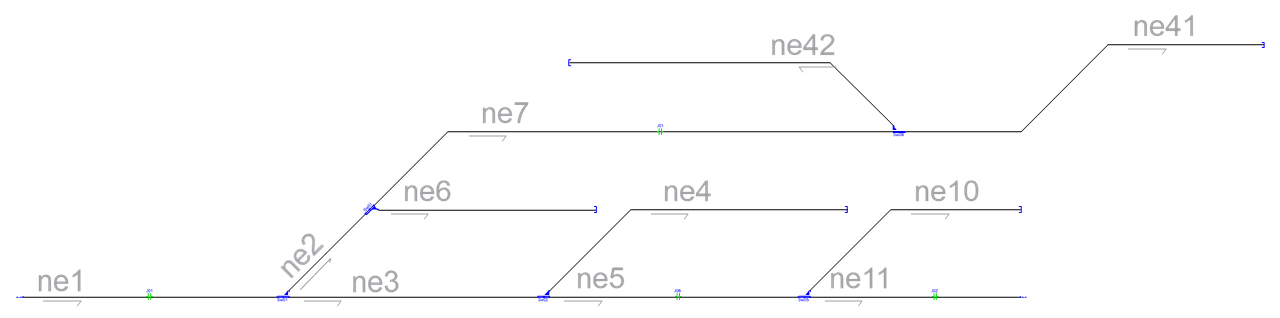
\includegraphics[width=1\textwidth]{resultados-obtenidos/ejemplo6/images/6_empty.png}
		\centering\caption{Topología ferroviaria del ejemplo 6 sin señalamiento.}
		\label{fig:EJ6_1}
	\end{figure}
	
	Para incrementar la dificultad del análisis y obtener resultados mas completos, se incluyeron finales de vías relativos y absolutos. No se incluyeron plataformas o cruces de vías.
